\section{The robustness was bought by knowing the density}
\label{sec:density}

The completeness result of \S\ref{sec:completeness:two} was obtained with the
sparse tracer's comoving number density pinned at the truth, which is the most
favourable case available. It is also the case that makes the mechanism work:
the completion converts a \emph{known} $n_0$ into a missing-host budget, and it
is that budget which keeps the two tracer priors distinguishable once their
observed hosts are gone. Taking the knowledge away should therefore matter, and
it does --- more than incompleteness itself.

We map the two-dimensional likelihood in $(\fagn, \lognzagn)$ at each rung of
the ladder, on a $\FreeGridF \times \FreeGridN$ grid over
$\lognzagn \in [\FreeRangeLo, \FreeRangeHi]$ with the expansion rate pinned at
the truth, and read every level of prior knowledge off that one likelihood as a
reweighting rather than a separate run: a delta function at the truth for the
anchored case, a Gaussian of width $\log_{10}(1+\epsilon)$ dex for a fractional
knowledge $\epsilon$, and a flat prior for no knowledge at all. Nothing else
changes --- the same mock, the same events, the same catalogs, the same targeted
injection sets --- so the comparison adds exactly one degree of freedom. No grid
cell is inadmissible anywhere in the map.

\subsection{The interaction is the result}
\label{sec:density:interaction}

Figure~\ref{fig:n0sig} gives the detection significance of the AGN-hosted
fraction, median$/\sigma$, across completeness and density knowledge. With the density known exactly, taking the survey from complete to
$C = \IncMeighteenC$ costs \FreeCostExact\% of the significance:
\FreeCompleteExactSig$\sigma$ becomes \FreeMeighteenExactSig$\sigma$, which is
the near-immunity of \S\ref{sec:completeness:two} seen through a different
statistic. With the density free, the same thinning costs \FreeCostFree\%:
\FreeCompleteFreeSig$\sigma$ becomes \FreeMeighteenFreeSig$\sigma$, and almost
all of that is spent in the very first step away from a complete catalog, where
the significance falls to \FreeMtwentyoneFreeSig$\sigma$.

Reading across a row gives what density knowledge buys; reading down a column
gives what completeness costs. Neither reading alone is the result --- the
interaction is. Completeness and density knowledge are not separable axes,
because the completion can substitute a modelled budget for missing hosts only
if it is told how many hosts there should be.

The practical threshold, though, is encouraging. Knowing \nzagn\ to
\FreePriorDexTen\ dex --- about 10\% --- costs almost nothing at any
completeness: \FreeCompleteExactSig$\sigma$ becomes
\FreeCompleteTenSig$\sigma$ at complete, and \FreeMeighteenExactSig$\sigma$
becomes \FreeMeighteenTenSig$\sigma$ at $C = \IncMeighteenC$. A 30\% prior costs
noticeably more (\FreeCompleteThirtySig$\sigma$ and
\FreeMeighteenThirtySig$\sigma$), and a factor-of-two prior --- entirely
plausible for a real AGN luminosity function --- already sits at
\FreeMeighteenFtwoSig$\sigma$ once the survey is incomplete. The measurement
survives realistic anchoring; it does not survive ignorance.

\begin{figure}
\centering
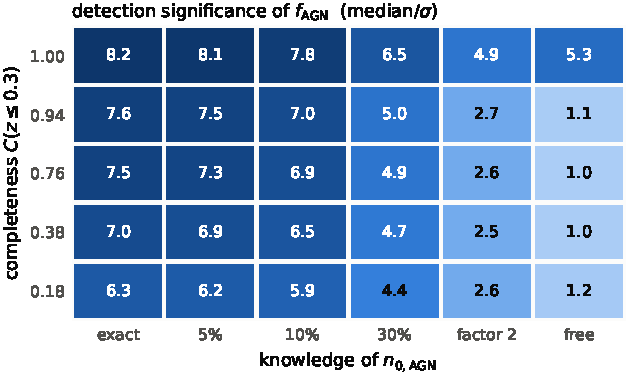
\includegraphics[width=\columnwidth]{figures/fig_n0_significance.pdf}
\caption{Detection significance of the AGN-hosted fraction, median$/\sigma$,
across survey completeness (rows) and prior knowledge of the sparse tracer's
comoving number density (columns). Every column is a reweighting of the same
likelihood grid, so the whole map comes from five grids. The two topmost entries
of the free column carry \FreeCompleteEdgeMass\% and
\FreeMtwentyoneEdgeMass\% of their density posterior against the low edge of the
scanned range and are partly statements about that range; the rest of the map is
not affected.
\label{fig:n0sig}}
\end{figure}


\subsection{Why the width alone would mislead}
\label{sec:density:width}

The 68\% half-width on \fagn\ (Table~\ref{tab:n0width}) is a poor summary here
and would give the wrong answer if quoted on its own. The narrowest entry
anywhere in the table is \FreeHwMin, and it belongs to the free-density column at
the complete rung ---
which is also among the least significant entries in that row, because the
posterior has collapsed onto small \fagn\ rather than measured it. That is why
the significance, not the width, is the headline: a posterior can be narrow and
centred anywhere.

\begin{deluxetable*}{ccccccc}
\tablecaption{68\% half-width on the AGN-hosted fraction across survey completeness (rows) and prior knowledge of the sparse tracer's comoving number density (columns), on the same grids as Figure~\ref{fig:n0sig}. The width alone is a misleading summary: its smallest entry anywhere in the table belongs to the free-density column at the complete rung, which is among the \emph{least} significant entries of that row. \label{tab:n0width}}
\tablehead{\colhead{$C$} & \multicolumn{6}{c}{knowledge of $n_{0,\rm AGN}$}\\ \colhead{} & \colhead{exact} & \colhead{$5\%$} & \colhead{$10\%$} & \colhead{$30\%$} & \colhead{factor 2} & \colhead{free}}
\startdata
1.00 & 0.053 & 0.053 & 0.054 & 0.055 & 0.052 & 0.033 \\
0.94 & 0.052 & 0.052 & 0.053 & 0.059 & 0.059 & 0.037 \\
0.76 & 0.052 & 0.052 & 0.054 & 0.060 & 0.062 & 0.042 \\
0.38 & 0.053 & 0.054 & 0.055 & 0.062 & 0.068 & 0.053 \\
0.18 & 0.058 & 0.059 & 0.061 & 0.071 & 0.087 & 0.091 \\
\enddata
\end{deluxetable*}


\subsection{The degeneracy, and which way it points}
\label{sec:density:degeneracy}

The correlation between the mixture weight and the density under a flat density
prior is \FreeCompleteRho\ at the complete rung and saturates at \FreeRhoMax\ as
soon as the survey thins (Figure~\ref{fig:n0deg}a). This is the anticipated
failure mode made quantitative: a missing AGN host and an AGN-hosted event both
explain an event in a pixel with no observed AGN, and once most hosts are
missing the two parameters are very nearly the same parameter. The joint region
is a curved band running from small \fagn\ at low density up toward the truth,
which at every rung lies at or just beyond the band's upper tip: the
flat-prior posterior stops short of it on both axes at once.

The direction of that band explains both of the fraction's biases at once. Under
a flat prior the density itself is recovered \emph{below} the truth at every
rung --- by \FreeCompleteNzeroOff, \FreeMtwentyoneNzeroOff,
\FreeMtwentyNzeroOff, \FreeMnineteenNzeroOff\ and \FreeMeighteenNzeroOff\ dex,
i.e.\ factors of \FreeCompletePrior\ down to \FreeMeighteenPrior\
(Figure~\ref{fig:n0deg}b). Pinned at the true density, the completion
manufactures a missing-AGN budget out of the shot noise of a sparse tracer and
pushes \fagn\ up, which is the high centre of \S\ref{sec:completeness:centres};
allowed to move, it kills that budget by driving the density down and pulls
\fagn\ below the truth instead. The two biases are the same mechanism seen from
opposite ends.

That also disposes of a tempting misreading of the map. Following the centre of
\fagn\ across the density priors, the truth falls inside the 68\% interval only
at intermediate prior widths --- the 30\% prior on most rungs, the
factor-of-two prior at the ends of the ladder --- and never in the free
column. This
is not evidence that an intermediate prior is the right one. The anchored bias
is high and the degeneracy pulls low, so \emph{some} intermediate prior width
necessarily crosses the truth, and where it crosses is set by the size of the
residual bias rather than by anything physical. The honest reading is that the
recovered fraction is a strong function of an assumption, over a range of
assumptions that are all defensible a priori --- which is itself the argument
for measuring \nzagn\ externally instead of marginalising over it.

\begin{figure*}
\centering

\includegraphics[width=\textwidth]{figures/fig_n0_degeneracy.pdf}
\caption{The degeneracy between the AGN-hosted fraction and the AGN comoving
number density, with the expansion rate pinned at the truth. \emph{(a)} 68\% and
90\% credible regions at the complete rung and at $C = \IncMeighteenC$; the
truth (cross) lies at or just beyond the upper tip of the band, which is why an
anchored density biases the fraction high and a free one biases it low. \emph{(b)} the
flat-prior density marginal at every rung; the density recovers below the truth
by \FreeCompleteNzeroOffAbs\ dex at complete, falling to
\FreeMeighteenNzeroOffAbs\ dex at the shallowest rung. At the two shallowest
survey depths the marginal keeps \FreeCompleteEdgeMass\% and
\FreeMtwentyoneEdgeMass\% of its mass against the low edge of the scanned range.
\label{fig:n0deg}}
\end{figure*}

\subsection{What this means for the programme}
\label{sec:density:consequences}

Three consequences follow, and they are requirements on the \emph{AGN survey}
rather than on the gravitational-wave data.

First, anchoring the tracer density to about 10\% is the design specification.
Below that the measurement degrades gracefully with survey depth; above it,
depth stops being the limiting factor.

Second, a fixed-density $\sigma(\fagn)$ must not be quoted as a forecast. At
fixed $n_0$ the width is nearly completeness-independent and reads as a robust
measurement; the same configuration with a factor-of-two density prior is a
\FreeMeighteenFtwoSig$\sigma$ result.

Third, in the incomplete regime the completion's missing-host budget is doing
more work than the observed hosts, and its amplitude is set entirely by $n_0$.
Everything downstream of the completion therefore inherits the density's
uncertainty, including the completeness-robustness of
\S\ref{sec:completeness:two}.
